\chapter{IMPLEMENTATION}

The implementation of models mentioned in Chapter 6 was performed using the Scikit-Learn library \cite{E}. For each code submission task, the dataset was split in the ratio 70:30 for training and testing. With respective to the hyper-parameters initialized for the individual models, 

\begin{itemize}
    \item The MLP regressor model was initialised with a single hidden layer with 100 neurons. The maximum iterations parameter was set to 5000. 
    \item The Random Forest Regressor was initialised with 100 estimators(decision trees).
    \item The Support Vector Regressor was initialised with linear kernel.
\end{itemize} 

% Talk about train test split

\section{METRICS}
 

\subsection{Mean Absolute Error (MAE)}

\[ MAE = \frac{\sum_{i=1}^{n}|t_i-y_i|}{n} \]

MAE is the mean of magnitude of difference between true value '$t_{i}$' and prediction '$y_{i}$' of 'n' observations.

\subsection{Root Mean Absolute Error (RMSE)}

\[ RMSE = \sqrt{\frac{\Sigma_{i=1}^{n}{|t_i-y_i|}^2}{n}} \]

RMSE is the square root of the mean of residuals (difference between between true value '$t_{i}$' and prediction '$y_{i}$') of 'n' observations 

\section{RESULTS}

The observed values of MAE and RMSE obtained for the different set of tasks are reported in sub sections 7.2.1 - 7.2.4. The values enclosed in brackets report scores observed with feature selection and the values not enclosed in brackets report scores observed without feature selection. 

\subsection{Selection Sort}

\begin{table}[h]
\centering
\caption{Results - Selection Sort}
\begin{tabular}{|c|c|c|}
\hline
\textbf{Model} & \textit{\textbf{MAE}} & \textit{\textbf{RMSE}} \\ \hline
\textbf{SVM}   & 1.35 \textbf{(1.27)}           & 1.94 \textbf{(1.84)}            \\ \hline
\textbf{MLP}   & 2.18 \textbf{(3.29)}           & 2.60 \textbf{(3.61)}             \\ \hline
\textbf{RF}    & 1.18 \textbf{(1.17)}           & 1.87 \textbf{(1.83)}            \\ \hline
\end{tabular}

\label{tab:selsort}
\end{table}

From table 7.1, we observe that Random Forest outperforms SVM and MLP in performance. 

\newpage

\subsection{First Negative Item in List}

\begin{table}[h]
\centering
\caption{Results - First Negative Item in List}
\begin{tabular}{|c|c|c|}
\hline
\textbf{Model} & \textit{\textbf{MAE}} & \textit{\textbf{RMSE}} \\ \hline
\textbf{SVM}   & 2.13 \textbf{(2.11)}           & 2.97 \textbf{(2.99)}            \\ \hline
\textbf{MLP}   & 3.02 \textbf{(3.13)}           & 3.80 \textbf{(3.90)}            \\ \hline
\textbf{RF}    & 1.60 \textbf{(1.64)}           & 2.15 \textbf{(2.20)}            \\ \hline
\end{tabular}

\label{tab:first-neg}
\end{table}

From table 7.2, we observe that Random Forest outperforms SVM and MLP in performance. 


\subsection{Largest Item in List}

\begin{table}[h]  
\centering
\caption{Results - Largest Item in List}
\begin{tabular}{|c|c|c|}
\hline
\textbf{Model} & \textit{\textbf{MAE}} & \textit{\textbf{RMSE}} \\ \hline
\textbf{SVM}   & 2.19 \textbf{(1.89)}           & 2.85 \textbf{(2.35)}            \\ \hline
\textbf{MLP}   & 2.73 \textbf{(3.28)}           & 3.61 \textbf{(4.23) }           \\ \hline
\textbf{RF}    & 1.51 \textbf{(1.47)}           & 2.10 \textbf{(2.07)}            \\ \hline
\end{tabular}

\label{tab:larg-list}
\end{table}

From table 7.3, we observe that Random Forest outperforms SVM and MLP in performance. 


\subsection{Unique Character count in a string}

\begin{table}[h]
\centering
\caption{Results - Unique Characters count in a string}
\begin{tabular}{|c|c|c|}
\hline
\textbf{Model} & \textit{\textbf{MAE}} & \textit{\textbf{RMSE}} \\ \hline
\textit{SVM} & 2.63 \textbf{(2.68)} & 3.19 \textbf{(3.23)} \\ \hline
\textit{MLP} & 3.11 \textbf{(2.71)} & 3.93 \textbf{(2.86)} \\ \hline
\textit{RF} & 2.16 \textbf{(2.19)} & 2.62 \textbf{(2.64)} \\ \hline
\end{tabular}

\label{tab:unique}
\end{table}

From table 7.4, we observe that Random Forest outperforms SVM and MLP in performance. 

\section{INFERENCE}

The number of features in the dataset is a comparitively smaller figure (only 17 features). And with feature selection, the number even reduces. Since random forest regressor is a ensemble of various decision trees, and the decision trees in turn output a score based on the feature value conditions(For instance when functions=3 for selection sort task, the decision tree will output a better score), random forest regressor fits well with the test data when compared to the other two models. Thus, Random forest regressor outperforms the linear support vector regressor and multi layer perceptron regressor. 

Since it is not possible to visualise the 17 features in 2 dimensions, the sum of all the features was plotted against the program score.
Figures 7.1 - 7.3 show the difference between the actual score (points plotted in orange) and the predicted score by the three regressors. The difference is represented as a line between the points. The three plots are for the selection sort task.

\begin{figure}[H]
\centering
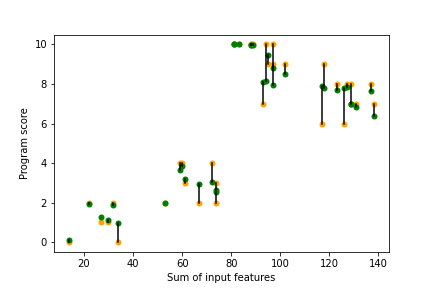
\includegraphics[scale=1.0]{./figures/ss_rf.png}
\caption{Actual score vs score predicted by Random Forest Regressor}
\label{fig_rf}
\end{figure}

\begin{figure}[H]
\centering
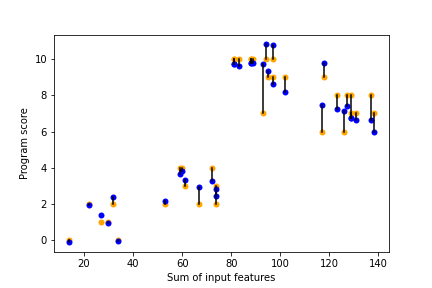
\includegraphics[scale=1.0]{./figures/ss_svr.png}
\caption{Actual score vs score predicted by Support Vector Regressor}
\label{fig_rf}
\end{figure}

\begin{figure}[H]
\centering
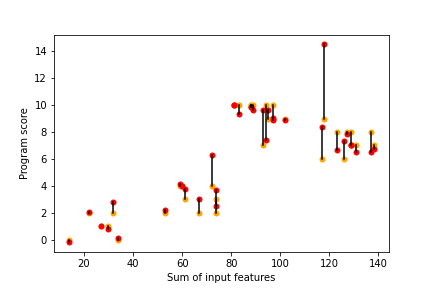
\includegraphics[scale=1.0]{./figures/ss_mlp.png}
\caption{Actual score vs score predicted by Multi Layer Perceptron Regressor}
\label{fig_rf}
\end{figure}

Also, while multi layer perceptron regressor and linear support vector regressor can output a score greater than 10 or lesser than 0, random forest regressor always outputs a score in the range of 0 to 10. This characteristic of random forest regressor is accounted by the decision trees which form the regressor. Since MLP regressor trains through backpropagation and support vector regressor tries to find the best hyperplane which contains maximum number of points, these models may output a score greater than 10. But in the case of random forest regressor, the model outputs a score based on the ensembling of various decision trees. The maximum score that can be awarded will be set as 10 and when a particular code submission passes all conditions(conditions are based on different feature values), that program will be graded with a score of 10. 

This can be observed in the figures 7.1-7.3. In case of random forest regressor as in figure 7.1, the scores always lie between zero and ten. Also the difference between actual and predicted values is lesser in general. In case of Support Vector Regressor as in figure 7.2, a couple of samples were given a score of over 10. In case of multi layer perceptron, one code sample was given a score over 14.

So, it can be inferred that Random Forest regressor is the most suited regression model for automatic grading of student programs.


